\section{Experiment 2 details}
\label{app:marker}

\subsection{Provenance}

Experiment 2 was run twice with the same design, generator, and scoring code. An earlier run used 24 histories (generation seed 23261011) and excluded a two-history pilot. The run reported in the main text uses 96 histories (generation seed 23261012) and excludes both the pilot and the 24-history run; its design document was hash-stamped on the experiment machine before the dataset was generated. Both runs scored every prompt (24-history run: 3,072 prompts, 2,272 distinct; 96-history run: 12,288 prompts, 8,544 distinct), with scoring seed 20261006, the checkpoint revisions of Appendix~\ref{app:provenance}, Python 3.13.5, an NVIDIA GeForce RTX 5080 with CUDA 13.0, and the int8 configurations of Experiment 1. Experiment 2 records candidate scores only, not generated answers. Artifact hashes are listed in the supplementary material.

Phi-4-mini was scored separately on the same 24-history dataset as an exploratory model extension, not as part of the prespecified Qwen/Gemma confirmation. Its pinned revision was \lit{cfbefacb99257ffa30c83adab238a50856ac3083}; it used the RTX 5080 with CUDA 13.0, int8 weights, and float16 activations. Its saved analysis recomputes exactly from all 3,072 score rows. As for the primary models, these are candidate-score results only and do not measure generated-answer accuracy.

\subsection{Templates and marker effects}

Table~\ref{tab:marker-templates} gives the four historical-line templates, Table~\ref{tab:marker} the marker effects and their interaction by order group, and Figure~\ref{fig:marker-effects} the underlying relevance.

\begin{table}[t]
\caption{The four historical-line templates of Experiment 2, shown for Nora. Each prompt has two such lines, one per entity, followed by the current-state block and query of Experiment 1.}
\label{tab:marker-templates}
\begin{center}
\small
\begin{tabular}{@{}l>{\raggedright\arraybackslash}p{0.33\linewidth}>{\raggedright\arraybackslash}p{0.40\linewidth}@{}}
\toprule
Construction & Marker absent & Marker present \\
\midrule
Superseded & \lit{Nora's badge was amber.} & \lit{Previously, Nora's badge was amber.} \\
Entity mention & \lit{Nora mentioned amber in an unrelated note.} & \lit{Previously, Nora mentioned amber in an unrelated note.} \\
\bottomrule
\end{tabular}
\end{center}
\end{table}

\begin{table}[t]
\caption{Marker effects, $R_{\text{present}}-R_{\text{absent}}$, and the marker-by-construction interaction (superseded minus entity-mention marker effect) in Experiment 2, in nats, with 95\% history-bootstrap intervals over 96 histories. The underlying $R$ values, their source/donor components, and the earlier 24-history run are in Appendix~\ref{app:marker}.}
\label{tab:marker}
\begin{center}
\small
\begin{tabular}{@{}llrrr@{}}
\toprule
Model & Order & Superseded & Entity mention & Interaction \\
\midrule
Qwen3-8B & All & −0.652 [−0.748, −0.560] & −1.734 [−1.934, −1.536] & 1.082 [0.850, 1.308] \\
Qwen3-8B & Aligned & −0.366 [−0.484, −0.243] & −1.000 [−1.164, −0.834] & 0.635 [0.427, 0.841] \\
Qwen3-8B & Reversed & −0.938 [−1.071, −0.804] & −2.469 [−2.746, −2.189] & 1.530 [1.208, 1.847] \\
\midrule
Gemma 3 4B & All & −0.950 [−1.062, −0.841] & −1.075 [−1.166, −0.986] & 0.125 [−0.012, 0.265] \\
Gemma 3 4B & Aligned & −0.963 [−1.100, −0.834] & −1.445 [−1.566, −1.326] & 0.482 [0.307, 0.655] \\
Gemma 3 4B & Reversed & −0.937 [−1.112, −0.767] & −0.705 [−0.833, −0.580] & −0.232 [−0.436, −0.027] \\
\bottomrule
\end{tabular}
\end{center}
\end{table}

\begin{figure}[t]
\begin{center}
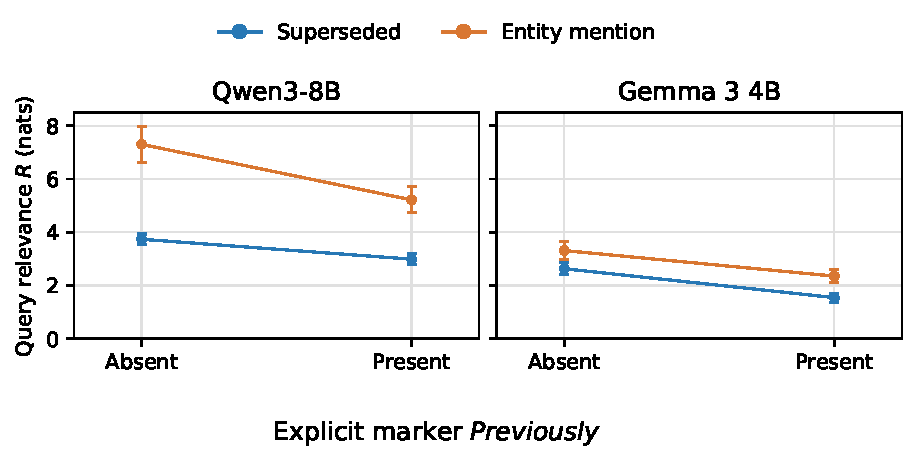
\includegraphics[width=0.9\linewidth]{figures/marker_by_construction.pdf}
\end{center}
\caption{Query relevance in Experiment 2 by marker and construction, separately for aligned (top) and reversed (bottom) order. Points are means over 96 histories; intervals are marginal 95\% history-bootstrap intervals. In Gemma the lines are further apart without the marker under aligned order and converge under reversed order, so the marker-by-construction interaction changes sign between order groups; paired marker effects and interactions are in Table~\ref{tab:marker}.}
\label{fig:marker-effects}
\end{figure}

\subsection{Query relevance and its components}

$E$ can be split into the change in the donor's score minus the change in the source's score. Applying the $R$ transformation to each part gives $R=R_{\text{donor}}-R_{\text{source}}$. Table~\ref{tab:d-decomposition} reports $R$ and both components in the 96-history run. With the marker, the donor component is smaller and the source component less negative, at the mean level, in both constructions and both models.

\begin{table}[h]
\caption{Overall $R$ and its donor and source components by construction and marker state in the 96-history run (nats).}
\label{tab:d-decomposition}
\begin{center}
\footnotesize
\begin{tabular}{@{}lllrrr@{}}
\toprule
Model & Construction & \lit{Previously} & $R$ & Donor component & Source component \\
\midrule
Qwen3-8B & Superseded & Absent & 3.486 [3.357, 3.628] & 1.622 [1.443, 1.810] & −1.864 [−2.075, −1.654] \\
Qwen3-8B & Superseded & Present & 2.834 [2.721, 2.946] & 1.448 [1.274, 1.621] & −1.386 [−1.581, −1.199] \\
Qwen3-8B & Entity mention & Absent & 6.545 [6.250, 6.866] & 3.106 [2.849, 3.363] & −3.438 [−3.743, −3.166] \\
Qwen3-8B & Entity mention & Present & 4.810 [4.619, 5.015] & 2.281 [2.087, 2.493] & −2.530 [−2.719, −2.345] \\
\midrule
Gemma 3 4B & Superseded & Absent & 2.502 [2.351, 2.663] & 1.244 [1.115, 1.374] & −1.258 [−1.425, −1.097] \\
Gemma 3 4B & Superseded & Present & 1.552 [1.453, 1.654] & 0.793 [0.666, 0.925] & −0.759 [−0.893, −0.620] \\
Gemma 3 4B & Entity mention & Absent & 3.409 [3.252, 3.575] & 1.633 [1.483, 1.783] & −1.776 [−1.935, −1.619] \\
Gemma 3 4B & Entity mention & Present & 2.334 [2.204, 2.474] & 1.104 [0.976, 1.246] & −1.230 [−1.373, −1.080] \\
\bottomrule
\end{tabular}
\end{center}
\end{table}

\subsection{The earlier 24-history run}

The 24-history run gave the same pattern as the 96-history run (Table~\ref{tab:d-marker24}): every marker effect is negative, Qwen's interaction is positive, and Gemma's interaction interval includes zero. Its $R$ decomposition and paired component changes are in Tables~\ref{tab:d-decomposition24} and~\ref{tab:d-paired}. The two runs are not pooled.

\begin{table}[h]
\caption{Marker effects and marker-by-construction interaction in the 24-history run (nats; 95\% history-bootstrap intervals).}
\label{tab:d-marker24}
\begin{center}
\small
\begin{tabular}{@{}llrrr@{}}
\toprule
Model & Order & Superseded & Entity mention & Interaction \\
\midrule
Qwen3-8B & All & −0.750 [−0.917, −0.590] & −2.087 [−2.410, −1.772] & 1.337 [0.976, 1.712] \\
Qwen3-8B & Aligned & −0.372 [−0.552, −0.187] & −1.298 [−1.580, −0.979] & 0.926 [0.581, 1.274] \\
Qwen3-8B & Reversed & −1.127 [−1.324, −0.939] & −2.876 [−3.354, −2.429] & 1.749 [1.236, 2.274] \\
\midrule
Gemma 3 4B & All & −1.085 [−1.308, −0.864] & −0.960 [−1.183, −0.727] & −0.125 [−0.390, 0.136] \\
Gemma 3 4B & Aligned & −1.100 [−1.359, −0.851] & −1.155 [−1.384, −0.915] & 0.055 [−0.233, 0.328] \\
Gemma 3 4B & Reversed & −1.069 [−1.372, −0.785] & −0.765 [−1.123, −0.387] & −0.304 [−0.753, 0.116] \\
\bottomrule
\end{tabular}
\end{center}
\end{table}

\begin{table}[h]
\caption{Overall $R$ and its donor and source components by construction and marker state in the 24-history run (nats).}
\label{tab:d-decomposition24}
\begin{center}
\footnotesize
\begin{tabular}{@{}lllrrr@{}}
\toprule
Model & Construction & \lit{Previously} & $R$ & Donor component & Source component \\
\midrule
Qwen3-8B & Superseded & Absent & 3.738 [3.536, 3.934] & 1.590 [1.118, 2.005] & −2.149 [−2.623, −1.705] \\
Qwen3-8B & Superseded & Present & 2.989 [2.791, 3.186] & 1.283 [0.832, 1.746] & −1.705 [−2.151, −1.242] \\
Qwen3-8B & Entity mention & Absent & 7.304 [6.629, 7.966] & 3.875 [3.477, 4.277] & −3.429 [−4.135, −2.764] \\
Qwen3-8B & Entity mention & Present & 5.217 [4.749, 5.705] & 2.540 [2.171, 2.917] & −2.677 [−3.193, −2.165] \\
\midrule
Gemma 3 4B & Superseded & Absent & 2.631 [2.409, 2.863] & 1.413 [1.170, 1.652] & −1.218 [−1.501, −0.934] \\
Gemma 3 4B & Superseded & Present & 1.546 [1.379, 1.714] & 0.685 [0.445, 0.932] & −0.861 [−1.115, −0.610] \\
Gemma 3 4B & Entity mention & Absent & 3.313 [2.975, 3.669] & 1.732 [1.427, 2.048] & −1.582 [−1.915, −1.276] \\
Gemma 3 4B & Entity mention & Present & 2.353 [2.114, 2.605] & 1.079 [0.874, 1.287] & −1.274 [−1.468, −1.068] \\
\bottomrule
\end{tabular}
\end{center}
\end{table}

\begin{table}[h]
\caption{Paired marker-induced changes (present minus absent) in the donor and source components in the 24-history run (nats); $\Delta R=\Delta R_{\text{donor}}-\Delta R_{\text{source}}$.}
\label{tab:d-paired}
\begin{center}
\small
\begin{tabular}{@{}lllrr@{}}
\toprule
Model & Order & Construction & $\Delta$ donor component & $\Delta$ source component \\
\midrule
Qwen3-8B & All & Superseded & −0.306 [−0.812, 0.237] & 0.443 [−0.100, 1.040] \\
Qwen3-8B & All & Entity mention & −1.335 [−1.640, −1.013] & 0.752 [0.323, 1.140] \\
Qwen3-8B & Aligned & Superseded & −0.286 [−0.840, 0.267] & 0.086 [−0.522, 0.704] \\
Qwen3-8B & Aligned & Entity mention & −0.810 [−1.328, −0.330] & 0.488 [−0.179, 1.070] \\
Qwen3-8B & Reversed & Superseded & −0.327 [−0.995, 0.399] & 0.800 [0.088, 1.557] \\
Qwen3-8B & Reversed & Entity mention & −1.859 [−2.283, −1.435] & 1.017 [0.480, 1.492] \\
\midrule
Gemma 3 4B & All & Superseded & −0.727 [−1.046, −0.420] & 0.357 [−0.009, 0.720] \\
Gemma 3 4B & All & Entity mention & −0.653 [−1.003, −0.310] & 0.307 [−0.021, 0.645] \\
Gemma 3 4B & Aligned & Superseded & −0.547 [−1.049, −0.015] & 0.553 [0.062, 1.085] \\
Gemma 3 4B & Aligned & Entity mention & −0.679 [−1.101, −0.245] & 0.475 [0.056, 0.909] \\
Gemma 3 4B & Reversed & Superseded & −0.907 [−1.298, −0.486] & 0.162 [−0.301, 0.629] \\
Gemma 3 4B & Reversed & Entity mention & −0.626 [−1.085, −0.207] & 0.139 [−0.285, 0.532] \\
\bottomrule
\end{tabular}
\end{center}
\end{table}

\subsection{Exploratory Phi-4-mini extension}

For Phi-4-mini, adding the explicit prefix \lit{Previously,} changed $R$ in the superseded construction by −1.355 nats (95\% CI [−1.561, −1.138]), from 5.146 [4.947, 5.362] without the marker to 3.791 [3.592, 4.004] with it. In the entity-mention construction, the marker effect was 0.145 [−0.018, 0.310], an unresolved change from 4.808 [4.557, 5.107] to 4.953 [4.677, 5.269]. The paired marker-by-construction interaction was −1.500 [−1.734, −1.264], indicating a larger reduction for the superseded construction in this model.

The order-stratified estimates show additional heterogeneity. Superseded marker effects were −1.227 [−1.412, −1.026] in aligned order and −1.483 [−1.758, −1.194] in reversed order. Entity-mention effects were −0.253 [−0.450, −0.059] aligned and 0.544 [0.384, 0.703] reversed. The corresponding interaction was −0.973 [−1.221, −0.714] aligned and −2.027 [−2.330, −1.725] reversed. These exploratory estimates indicate construction- and order-dependent score effects for Phi-4-mini; they do not establish a general model-family pattern or identify a mechanism. They are effects of adding the literal prefix, not evidence of active suppression. No answer-generation accuracy was collected in this candidate-scoring run.

\begin{table}[h]
\caption{Exploratory Phi-4-mini marker-confirmation estimates (nats; 24 histories; 95\% history-bootstrap intervals). Marker effect is present minus absent; interaction is the superseded marker effect minus the entity-mention marker effect.}
\label{tab:d-phi-marker}
\begin{center}
\small
\begin{tabular}{@{}lrrr@{}}
\toprule
Order & Superseded marker effect & Entity-mention marker effect & Interaction \\
\midrule
All & −1.355 [−1.561, −1.138] & 0.145 [−0.018, 0.310] & −1.500 [−1.734, −1.264] \\
Aligned & −1.227 [−1.412, −1.026] & −0.253 [−0.450, −0.059] & −0.973 [−1.221, −0.714] \\
Reversed & −1.483 [−1.758, −1.194] & 0.544 [0.384, 0.703] & −2.027 [−2.330, −1.725] \\
\bottomrule
\end{tabular}
\end{center}
\end{table}

\FloatBarrier
